\chapter{编队控制器设计}
\label{chap:controller_design}
第\ref{chap:formation_dynamic_equ}章中介绍了无人机双机编队的动力学模型,并将无人机运动分为竖直平面以及水平平面;方程组\ref{fol_motion_eauation1}水平平面的直接输入量为$\Psi$的期望值,竖直平面的
直接输入量为$\theta$和$V$的期望值。整体的控制逻辑框图如下图所示:
\begin{figure}[H]
    \centering
    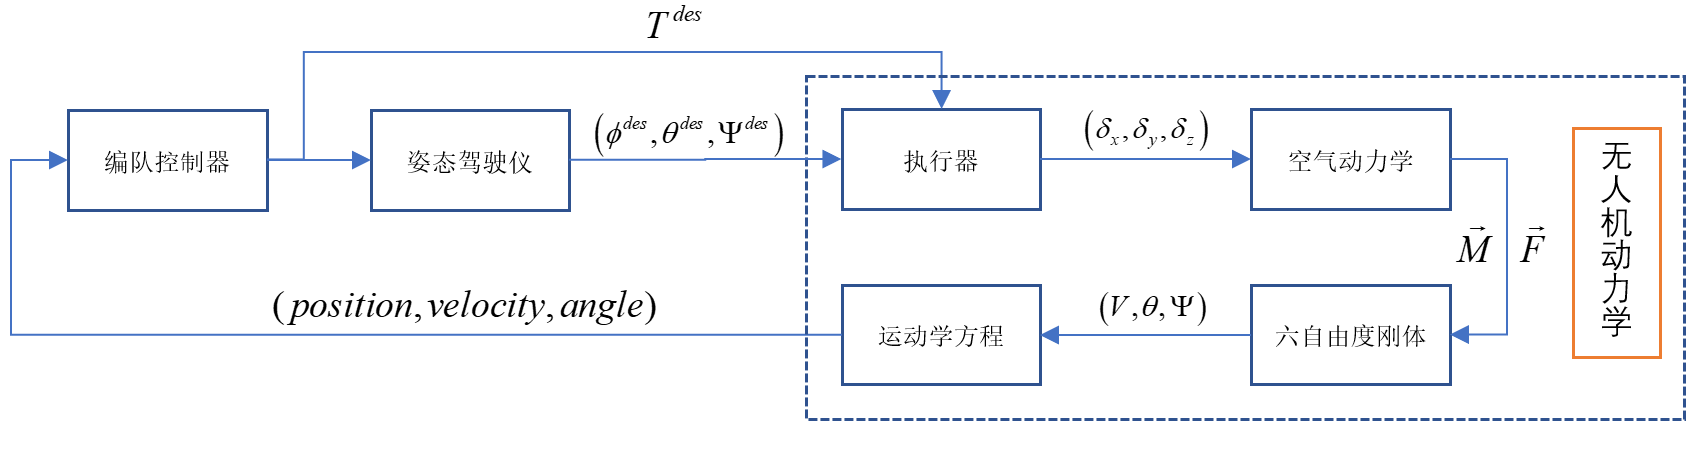
\includegraphics[width=0.85\textwidth]{figures/c3/c3-overview_controller.png}
    \caption{控制逻辑框图}\label{fig:c3-overview_controller}
\end{figure}
编队控制器的输入为定义的误差量,输出为无人机自动驾驶仪的内环输入值,即期望推力$T^{des}$,期望姿态$\Phi^{des},\theta^{des}$,偏航期望值$\Psi^{des}$将由内环姿态
自动驾驶仪按照协调转弯条件计算得到。本章的剩余部分将分别设计竖直平面以及水平平面的控制器。

需要说明的是:本章前两节先假设大气静止,设计无风条件下的编队控制器,第三节再引入风的干扰,并做相应处理。根据第二章的坐标系的定义,此假设将使得航迹坐标系与速度坐标系重合,又因为“无侧滑条件”(也称作协调转弯条件,BTT)的引入,机体二维水平平面坐标系$O_bx_by_b$将与前二者的水平平面坐标系($O_kx_ky_k$和$O_ax_ay_a$)重合。进而控制器产生的控制量与执行机构恰好对应,因此前两节之中,上述三种二维平面坐标系将不做区分。下面将选取航迹坐标系设计编队控制器。
\section{水平平面编队控制器设计}
\subsection{误差定义}
导航与制导的本质是控制地速的方向,实现手段是产生垂直于地速方向的法向加速度$a_{y_k}^{des}$;因而本章中误差以及控制量全部定义在航迹坐标系$O_kx_ky_kz_k$之中。但编队控制器不仅要控制速度的方向,还要控制速度的大小,以实现与领机的同步飞行。编队控制的最终目标为:
\begin{enumerate}
    \item 从机速度方向与领机的速度方向一致。
    \item 从机的速度大小与领机的速度大小一致。
    \item 从机的位置与从机的期望位置一致。
\end{enumerate}
此处产生三种误差类型,这三类误差均投影在从机航迹坐标系$O_kx_ky_kz_k$之中,便于之后对应要控制的物理量产生控制量:
\begin{enumerate}
    \item 领机与从机2维速度方向误差$\eta$,参见图\ref{fig:c02-2d_level_motion}。%TODO:记得改一下图,与之对应
    \item 领机与从机速度(地速$V_g$)大小误差$|V_g|^{err}$。
    \item 领机与期望位置3维误差$(P_{x_k}^{err},P_{y_k}^{err},P_{z_k}^{err})$
\end{enumerate}
因而此处水平平面的编队控制器的控制的任务是消除水平平面内的位置误差、速度大小以及速度方向误差,前两者在$O_kx_k$轴的分量需通过期望速度大小${|V|}_{x_k}^{des}$消除;前两者在$O_ky_k$轴
的分量,以及速度方向误差须通过期望法向加速度$a_{y_k}^{des}$消除。值得注意的是:实际上此处的速度方向误差代表了航迹系内的两分量之比值,实际上与角度误差代表同一误差,但是由于航迹系$O_kx_k$轴
的期望速度时刻变化,而所需的速度方向须按照领机速度方向一致,因而要控制速度的方向,而不是单纯的$O_kx_k$轴的速度分量。
\subsection{航迹系x轴方向控制器}
航迹系$O_kx_k$轴方向的控制器的输入为速度大小误差以及位置误差沿本轴分量的混合,控制器选用增量式离散$PID$控制器,最终的控制量的输出为航迹坐标系$O_kx_k$轴期望速度大小${|V|}_{x_k}^{des}$。控制器的表达式为:
\begin{equation}
    \left\{
    \begin{array}{l}
        |V_g|^{err}(k)=|V_g^{l}|(k)-|V_g^{f}|(k)\\
        P_{x_k}^{err}(k)=P_{x_g}^{des}(k)-P_{x_g}^{f}(k)\\
        e_{x_k}(k)=K_V|V_g|^{err}(k)+K_{Px}P_{x_k}^{err}(k)\\
        \begin{aligned}
        \Delta{|V|}_{x_k}^{des}(k)=&K_{p}^{xmix}[e_{x_k}(k)-e_{x_k}(k-1)]+K_{i}^{xmix}e_{x_k}(k)+\\
        &K_{d}^{xmix}[e_{x_k}(k)-2e_{x_k}(k-1)+e_{x_k}(k-2)]
        \end{aligned}
        \\
        {|V|}_{x_k}^{des}(k)=\Delta{|V|}_{x_k}^{des}(k)+{|V|}_{x_k}^{des}(k-1)
    \end{array}
    \right .
    \label{xk_vel_gen_equ}
\end{equation}
其中,前3式定义了混合误差形式,实际为速度误差与位置误差的线性叠加。后2式表示了最终的期望速度大小的产生。$k$为控制器第$k$次采样计算;$K_V,K_P$为误差线性混合常;$K_{p}^{xmix},K_{i}^{xmix},K_{d}^{xmix}$为增量式离散
$PID$控制器参数。

此处产生的期望速度大小,并不能直接为内环姿态驾驶仪所响应,需要经过竖直平面控制器的计算,位置误差$P_{z_k}^{err}$共同产生期望油门以及期望俯仰角。
\subsection{航迹系y轴方向控制器}
航迹系$O_ky_k$轴方向的控制器的输入为速度方向误差$\eta$以及位置误差的混合,类似于航迹系$O_kx_k$轴方向的控制器,控制器也选用增量式离散$PID$控制器,最终的输出为无人机滚转角期望值。
由图\ref{fig:c02-2d_level_motion}可得到:
\begin{equation}
    \eta^f=\Psi^l-\Psi^f
    \label{yaw_error}
\end{equation}
上式得到的是无人机速度方向的角度误差;

再考虑如图所示的无人机二维平面转弯运动:
\begin{figure}[H]
    \centering
    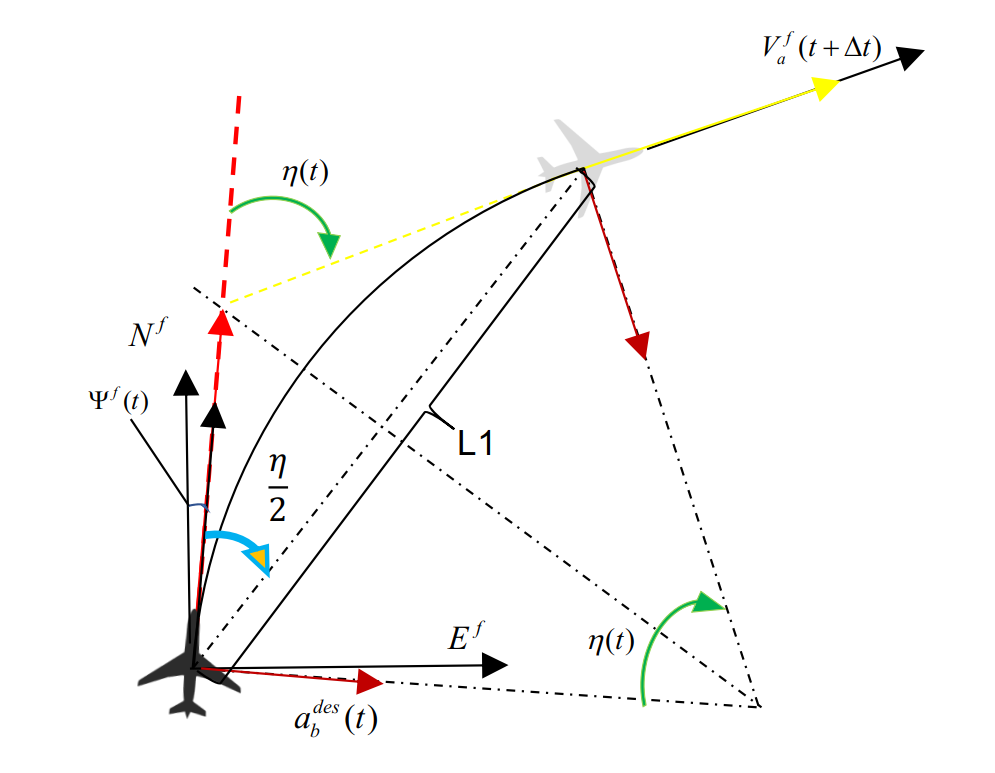
\includegraphics[width=0.5\textwidth]{figures/c3/c3-BTT.png}
    \caption{无人机二维平面转弯运动}\label{fig:c3-BTT}
\end{figure}
由于飞机速度的动力学惯性很大,在微分时间$\Delta t$时间内,速度的变化量可以忽略不计;在此时间内的偏航角增量为$\Delta\eta$,按照图中的几何关系,不难得到:
\begin{equation}
    a_{y_k}=V_g\dot{\eta}
    \label{btt_dot}
\end{equation}
上式即无人机期望偏航角速度与期望法向加速度关系。类似于上一节,定义混合误差为角度误差以及距离误差的线型混合。
再利用上一小节提出的增量式离散$PID$控制器,再综合式\ref{yaw_error},可得混合误差到期望法向加速度的表达式为:
\begin{equation}
    \left\{
        \begin{array}{l}
            \eta^f(k)=\Psi^l(k)-\Psi^f(k)\\
            P_{y_k}^{err}(k)=P_{y_g}^{des}(k)-P_{y_g}^{f}(k)\\
            e_{y_k}(k)=K_{\eta}\eta^f(k)+K_{Py}P_{y_k}^{err}(k)\\
                \begin{aligned}
                \Delta\dot{\Psi}^{des}(k)=&K_{p}^{ymix}[e_{y_k}(k)-e_{y_k}(k-1)]+K_{i}^{ymix}e_{y_k}(k)+\\
                &K_{d}^{ymix}[e_{y_k}(k)-2e_{y_k}(k-1)+e_{y_k}(k-2)]
                \end{aligned}\\
            \dot{\Psi}^{des}(k)=\Delta\dot{\Psi}^{des}(k)+\dot{\Psi}^{des}(k-1)\\
            \dot{\eta}^{des}(k)=-\dot{\Psi}^{des}(k)\\
            a_{y_k}^{des}(k)=-V_g^{f}(k)\dot{\eta}^{des}(k)
    \end{array}
\right .
    \label{angle_controller}
\end{equation}
上式得到的是期望法向加速度,再利用协调转弯(BTT)条件,将期望法向加速度,转化为期望滚转角:
\begin{equation}
    \tan\Phi^{des}(k)=\frac{a_{y_k}^{des}(k)}{g}
    \label{btt_a2roll}
\end{equation}
其中,$g$为当地重力加速度常量。至此,水平平面面内可计算得到无人机的期望滚转角$\Phi^{des}$以及期望速度大小$|V|_{x_k}^{des}$
\section{竖直平面编队控制器设计}
竖直平面编队控制器的输入为期望速度大小$|V|_{x_k}^{des}$以及期望高度(实际代表了高度误差$P_{z_b}^{err}$),输出为期望俯仰角$\theta^{des}$以及期望推力$T^{des}$。控制器选用基于能量的总能量控制法
(total energy control system,$TECS$)。固定翼无人机的速度控制和高度控制是耦合的,即单独控制高度或速度时,另一个未被控制量将会发生变化:
下面通过飞机飞行动力学纵向运动方程简单说明:
\\方程组\ref{fol_motion_eauation1}的第三式说明:飞机高度方向的变化率与地速大以及俯仰角大小有关,且为正相关。
\\根据飞机飞行动力学,无人机纵向运动质心运动的动力学方程为:
\begin{equation}
    \left\{
    \begin{aligned}
    &m \frac{\mathrm{d} V}{\mathrm{d} t}=T \cos (\alpha+\varphi) \cos \beta-D-m g \sin \gamma\\
    &m V \cos \gamma \frac{\mathrm{d} \chi}{\mathrm{d} t}=T[\sin (\alpha+\varphi) \sin \mu-\cos (\alpha+\varphi) \sin \beta \cos \mu]+C \cos \mu+L \sin \mu\\
    &-m V \frac{\mathrm{d} \gamma}{\mathrm{d} t}=T[-\sin (\alpha+\varphi) \cos \mu-\cos (\alpha+\varphi) \sin \beta \sin \mu]+\operatorname{Csin} \mu-L \cos \mu+m g \cos \gamma
    \end{aligned}
    \right .
    \label{point_dynamaic}
\end{equation}
其中,$\alpha,\mu,\phi$分别为迎角,速度滚转角以及发动机安装角。
根据之前的假设,可以将第一式近似作:
\begin{equation}
    m \frac{\mathrm{d} V}{\mathrm{d} t}=T-D-m g \sin \theta
    \label{1st_point_dynamaic}
\end{equation}
综合\ref{1st_point_dynamaic}、\ref{fol_motion_eauation1}两式,可以得到如下关于速度以及高度通道的控制逻辑图:
\begin{figure}[H]
    \centering
    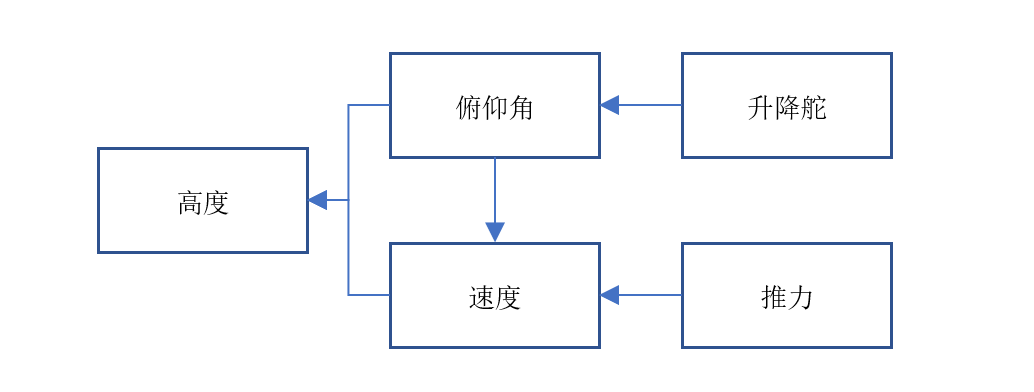
\includegraphics[width=0.75\textwidth]{figures/c3/relation_theta_thrust}
    \caption{速度以及高度通道的控制逻辑图}\label{fig:relation_theta_thrust}
\end{figure}
因而速度和高度需要同时考虑,相应的,期望俯仰角以及推力也需要同时计算。$TECS$控制器正是为此种情况设计的:%TODO:需要添加引用
所谓总能量控制(total energy control)是将无人机的速度以及高度计算得到相应的动能以及势能作为直接控制对象,应用PID控制器对动能与势能的和(total energy)
以及动能与势能的转化(total energy balance)进行控制,计算得到无人机期望俯仰角以及期望推力的控制器。飞机作为一个动力学系统,其机械能来自推力做功的输入,因而总能量控制对应着期望推力;与之对应的俯仰角控制是能量守恒的,
可作为动能向势能(反之亦然)的转化途径,对此种能量转化的控制对应着期望俯仰角。下面简要介绍$TECS$控制器的计算过程:
\\
无人机的总能量为:
\begin{equation}
    E_T=\frac{1}{2}mV_T^2+mgh
    \label{ET}
\end{equation}
对上式两边微分,可得到总能量变化率:
\begin{equation}
    \dot{E_T}=mV_T\dot{V_T}+mg\dot{h}
    \label{ET_rate}
\end{equation}
由此可得单位总能量变化率:
\begin{equation}
    \dot{E}=\frac{\dot{E}_{T}}{m g V_{T}}=\frac{\dot{V}_{T}}{g}+\frac{\dot{h}}{V_{T}}=\frac{\dot{V}_{T}}{g}+\sin \gamma
    \label{specif_ET_rate}
\end{equation}
更换式\ref{point_dynamaic}第一式形式,可得到:
\begin{equation}
    T-D=m g\left(\frac{\dot{V}_{T}}{g}+\sin \gamma\right)
    \label{point_dynamaic_change}
\end{equation}
由此可得:
\begin{equation}
    \Delta T=m g\left(\frac{\dot{V}_{T}}{g}+sin\gamma\right)
    \label{thrust}
\end{equation}
关于能量转化,定义:
\begin{equation}
    B=m g h-\frac{1}{2} m V_{T}^{2}
\end{equation}
能量转化率为:
\begin{equation}
\dot{B}=sin\gamma-\frac{\dot{V}_{T}}{g}
\end{equation}
这里参照开源软件$PX4$内部的TECS控制器设计方法,总能量环和能量分配环的控制逻辑框图如下所示:
\begin{figure}[H]
    \centering
    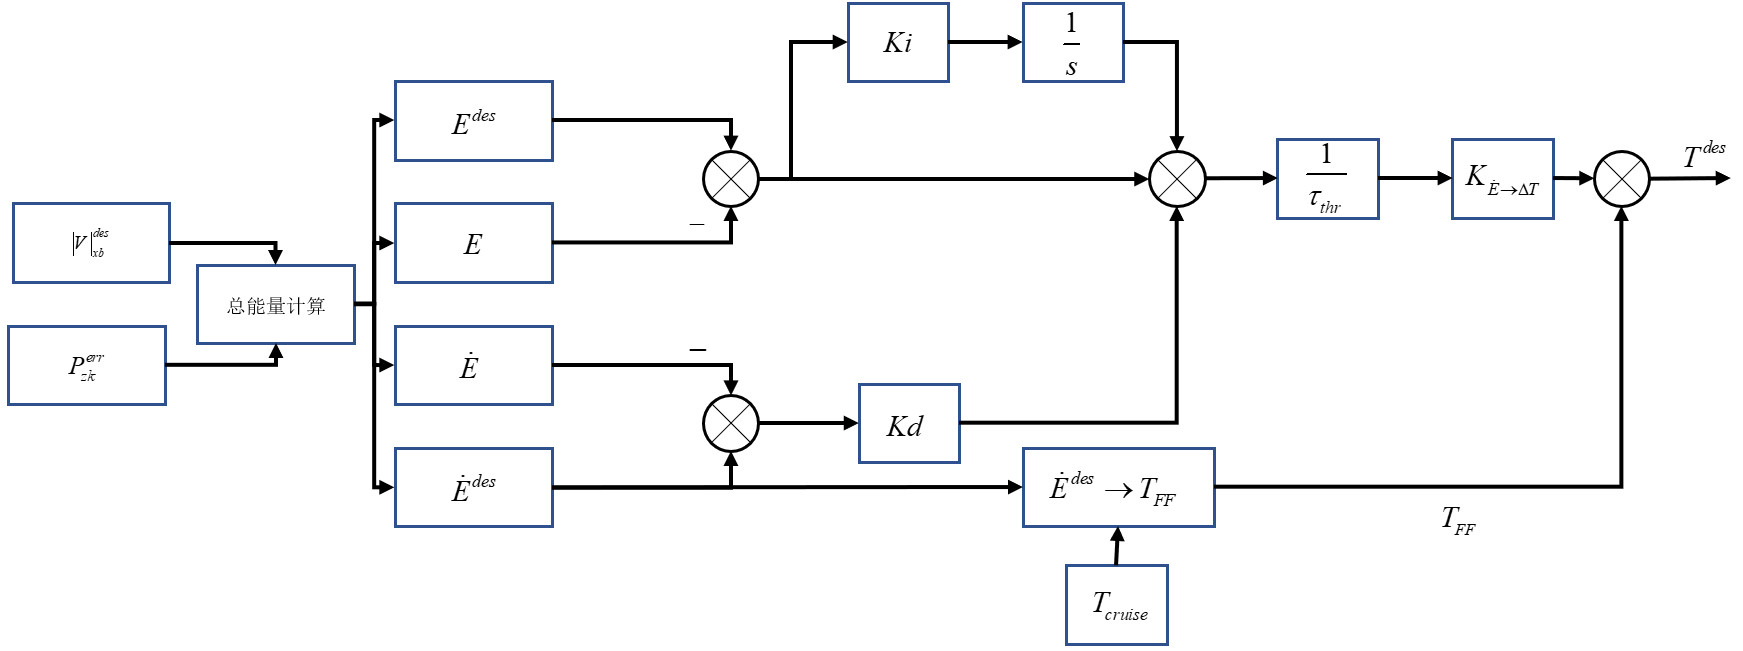
\includegraphics[width=0.9\textwidth]{figures/c3/TECS_throttle.jpg}
    \caption{总能量环}\label{fig:total_energy}
\end{figure}
\begin{figure}[H]
    \centering
    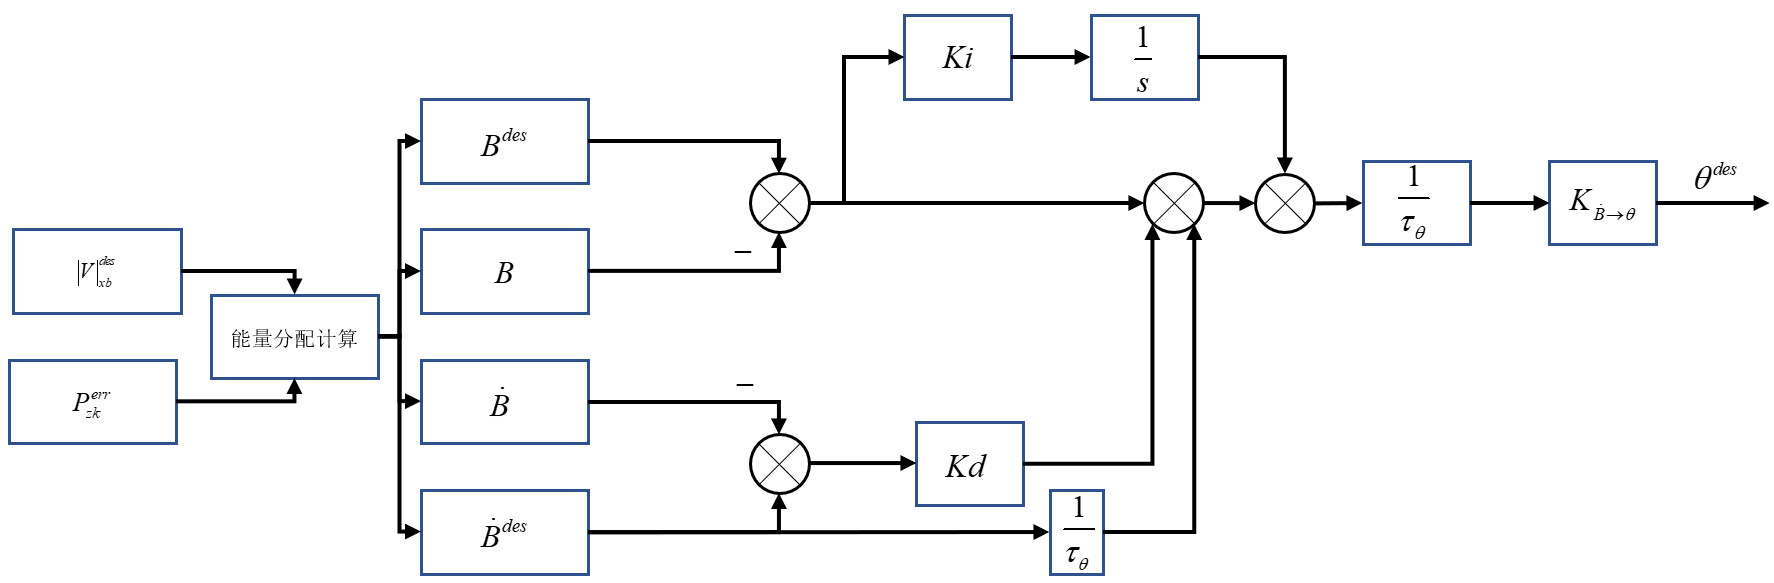
\includegraphics[width=0.9\textwidth]{figures/c3/TECS_pitch.jpg}
    \caption{能量分配环}\label{fig:balance_energy}
\end{figure}
图\ref{fig:total_energy}中,$K_i,K_d,T_{FF},\tau_{thr},K_{\dot{E}\rightarrow\Delta T}$分别为积分项,微分项比例系数,油门前馈项,油门时间常数以及比例向项系数。
图\ref{fig:balance_energy}中,$K_i,K_d,\tau_{\theta},K_{\dot{B}\rightarrow\Delta \theta}$分别为积分项,微分项比例系数,俯仰角时间常数以及比例向项系数。

至此,来自水平平面的期望速度$|V|_{x_k}^{des}$以及纵向平面的位置误差$P_{z_k}^{err}$将转化为期望俯仰角以及期望推力进入内环姿态驾驶仪;水平平面编队控制器
产生的期望滚转角也将进入姿态驾驶仪内环。内环姿态自动驾驶仪首先按照无侧滑条件得出期望偏航角速度$\dot{\Phi}^{des}$,然后再利用串级PID分角速度环,角
加速度环计算得到期望的执行机构的偏转角度。但现在的编队控制器还不足以直接用来进行编队控制实现,还需要经过一定的工程处理,详见下一节。
\section{实际应用时的考虑}
在实际应用编队控制器时,按照已有的经验,应主要考虑以下几个方面:
\begin{enumerate}
    \item 在无人机距离期望位置较远以及相对较近时,控制的目的是不完全一致的;应根据不同的控制需求分段设计控制律。
    \item 无人机的空速与地速差距较大(风速很大)时,地速与空速方向不能简单认为一致,应分析之后做相应的处理。
    \item 考虑到无人机各个动力学量的范围,应按照前期对于飞行平台飞行性能计算的结果对控制器计算过程中的各个物理量进行实际限幅。
    \item 无人机原始信息两量测噪声问题,应设计便于使用的滤波器加以滤波。
\end{enumerate}
下面按照上述问题介绍相应的解决方法:

\subsection{编队控制器分段设计} 
在位置误差较大时,编队控制器的主要目的应为:以最大速度飞行,迅速减小距离误差;此时无人机速度的期望方向应时刻指向期望点而并非领机的速度方向。选择水平距离误差大小作为分段控制器的分段依据,定义水平距离误差为$|P|_{2d}^{err}(k)=\sqrt{[P_{x_k}^{err}(k)]^2+[P_{y_k}^{err}(k)]^2}$,决断距离记作$|P_0|_{2d}^{err}$。于是可以得到以下期望速度的表达式:
\begin{equation}
    |V|_{x_k}^{des}(k)=
    \begin{cases}
        V_{max}^f& |P|_{2d}^{err}(k)>|P_0|_{2d}^{err}\\
        \Delta{|V|}_{x_k}^{des}(k)+{|V|}_{x_k}^{des}(k-1)& |P|_{2d}^{err}(k)\leq|P_0|_{2d}^{err}
    \end{cases}
    \end{equation}
第二阶段的期望速度速度产生详见式\ref{xk_vel_gen_equ}。
关于此阶段的法向加速度的产生,此处使用××等人提出的L1控制器,将L1距离选为从机当前位置与期望位置的距离误差。其表达式如下:
\begin{equation}
    a_{y_k}^{des}(k)=
    \begin{cases}
        2\frac{V^2}{L_1}\sin{\frac{\eta}{2}}& |P|_{2d}^{err}(k)>|P_0|_{2d}^{err}\\
        -V_g^{f}(k)\dot{\eta}^{des}(k)& |P|_{2d}^{err}(k)\leq|P_0|_{2d}^{err}
    \end{cases}
    \end{equation}
上式中各运动学量参见图\ref{fig:c3-BTT},第二阶段法向加速度的产生详见式\ref{angle_controller}。再配合固定翼无人机协调转弯条件(式\ref{btt_a2roll}),可得到分段之后的期望滚转角。
\subsection{风速较大时的处理} 
\subsubsection*{风速因素对于编队控制器的影响分析}
无论导航与制导还是编队的期望速度均是对无人机的地速而言的。当内环姿态驾驶仪以无侧滑条件为基础时,若控制效果较好,则可保证侧滑角$\beta\approx 0$,即:无人机在水平二维平面运动时,空速方向与机身纵轴在同一竖直平面内。因而飞机在平飞时,空速方向几乎与机身纵轴重合。无论有风还是无风,均有上述结论。

参照图\ref{fig:c02-2d_level_motion},当风速$V_{wind}^f$较小时,空速与地速几乎重合,且等大,此时直接将空速方向认为与空速方向一致,进而与机体方向一致的做法是可行的:前文提出的位置、角度以及速度误差均投影在航迹系$O_kx_ky_kz_b$中,所产生的修正信号$|V|_{x_k}^{des}(k),a_{y_k}^{des}(k)$与体轴系的$O_bx_b$以及$O_by_b$几乎重合,i控制机构(油门,副翼)直接相应控制信号即可,符合前文的设计。

但当风速较大时(例如,风速大小已经超过了地速的$\frac{1}{3}$,且与飞机地速有一定的角度),则会出现如下图所示的情况:
\begin{figure}[H]
    \centering
    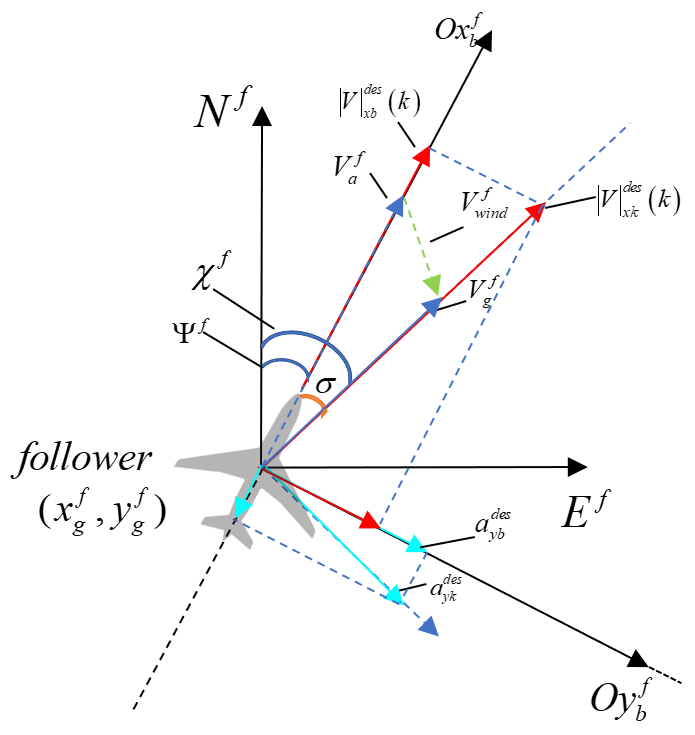
\includegraphics[width=0.5\textwidth]{figures/c3/heavy_wind.png}
    \caption{空速与地速之差较大}\label{fig:heavy_wind}
\end{figure}
图中,风速的大小以及方向已经不能忽略不计,可以得出。原始产生在航迹坐标系$O_kx_ky_kz_k$中的期望速度以及期望与执行机构(油门以及副翼)所在的机体系已有大小为$\sigma$的夹角。
\subsubsection*{风速较大时的改进}
如图\ref{fig:heavy_wind}所示,原始在航迹坐标系之中产生的控制量的期望值若要在机体系之中产生正确的相应,需要进行相应的坐标变换。
\begin{equation}
    \left[
    \begin{matrix}
        control\_input\_x_b(k)\\
        control\_input\_x_y(k)
    \end{matrix}
    \right]
    =  
    \left[  
    \begin{matrix}
        cos\sigma& -sin\sigma\\
        sin\sigma& cos\sigma
    \end{matrix}
    \right]
    \left[
        \begin{matrix}
            |V|_{x_k}^{des}(k)\\
            a_{y_k}^{des}(k)
        \end{matrix}
        \right]
\end{equation}
但是由于机体系两个通道所能够接受的的控制量并不是一致的,需要进行工程化处理:
\begin{equation}
    \left\{
        \begin{aligned}
            &control\_input\_x_b(k)=cos\sigma|V|_{x_k}^{des}(k)+\sum_{n=1}^k\{-sin[\sigma(n)]a_{y_k}^{des}(n)T\}\\
            &control\_input\_x_y(k)=\frac{1}{T}\{sin[\sigma(k)|V|_{x_k}^{des}(k)]-sin[\sigma(k-1)|V|_{x_k}^{des}(k-1)]\}+cos\sigma a_{y_k}^{des}(k)
        \end{aligned}
    \right .
\end{equation}
上式中,$T$是控制时间间隔。实际应用时上式中的微分项要考虑低通滤波以及时间间隔问题,积分项应考虑积分饱和问题。
\subsection{无人机飞行性能限幅设计}
考虑到实际系统各个环节的有界性问题,需要按照无人机气动外形尺寸以及基本飞机空气动力学,计算得出的无人机飞行性能参数,作为实际控制时的各个环节物理量的限幅依据。表\ref{tab:takeoff_performance}-\ref{tab:sink_performance}展示了飞机部分飞行性能:
\begin{table}[H]
    \centering
    \caption{无人机起飞、爬升性能} \label{tab:takeoff_performance}
    \begin{tabular*}{0.9\textwidth}{@{\extracolsep{\fill}}c|ccccccc}
    \toprule
        飞行性能&抬轮速度&起飞速度&滑跑距离&起飞时间
        &爬升率&爬升角
        \\
    \midrule
        值&$4.82m/s$&$5.52m/s$&$16.45m$&$7.36s$
        &$5.99m/s$&$31.21°$\\
    \bottomrule
\end{tabular*}
\end{table}
\begin{table}[H]
    \centering
    \caption{无人机平飞性能} \label{tab:task_performance}
    \begin{tabular*}{0.9\textwidth}{@{\extracolsep{\fill}}c|cccc}
    \toprule
        飞行性能&平定常飞空速&最大空速&最小空速&失速迎角%TODO:需要有最大前项加速度
        \\
    \midrule
        值&$11.52m/s$&$43.76m/s$&$4.60m/s$&$9.94°$\\
    \bottomrule
\end{tabular*}
\end{table}
\begin{table}[H]
    \centering
    \caption{无人机机动性能} \label{tab:motive_performance}
    \begin{tabular*}{0.9\textwidth}{@{\extracolsep{\fill}}c|ccccc}
    \toprule
        飞行性能&转弯速率&转弯半径&转弯时间&法向过载系数&最大滚转角%TODO:需要有最大滚转角速度
        \\
    \midrule
        值&$11.56m/s$&$14.31m/s$&$7.80s$&$1.38$&$43.56°$\\
    \bottomrule
\end{tabular*}
\end{table}
\begin{table}[H]
    \centering
    \caption{无人机下降、爬降落性能} \label{tab:sink_performance}
    \begin{tabular*}{0.9\textwidth}{@{\extracolsep{\fill}}c|cccc}
    \toprule
        飞行性能&下降率&下降角&降落速度&滑跑距离
        \\
    \midrule
        值&$10.19m/s$&$60.15m/s$&$5.89m/s$&$14.81m$
        \\
    \bottomrule
\end{tabular*}
\end{table}
\subsection{原始数据滤波器设计}
此处所涉及的原始数据,主要是来自领机以及从机的空速计测量的空速信息。此处使用一阶低通滤波器来实现对于空速信息的滤波。下面简单介绍一阶低通滤波器:
一阶低通滤波器又称作一阶惯性滤波器,传递函数形式为标准一阶惯性环节:
\begin{equation}
    V_0=\frac{1}{1+\tau j\omega}
\end{equation}
其中$\tau$是时间常数。转换成时域形式:
\begin{equation}
    V_0=V_i -\tau\frac{dV_0}{dt}
\end{equation}
离散化之后:
\begin{equation}
    V_0(k)=\frac{V_i(k)+\frac{\tau}{T}V_0(k-1)}{1+\frac{\tau}{T}}
\end{equation}
其中,$T$为控制器时间间隔,$T=\frac{1}{f}$。
此种滤波器在使用时需要注意时间常数的选择,时间常数过大,虽然数据波形会相对平滑,但是滞后较为严重。
